\section{Reactive Design Patterns}

Dieser Teil der Arbeit beschäftigt sich mit Reactive Design Patterns. Dabei handelt es sich nicht um gänzlich neue Design Patterns, sondern vielmehr um Patterns, die sich für die Entwicklung reaktiver Systeme als nützlich erweisen. Der Fokus soll vorallem auf Patterns liegen, die die Eigenschaften reaktiver Anwendungen unterstützen.

\subsection{Observable Pattern}
Das reaktive Observable Pattern stammt aus dem Hause Microsoft und wurde von Erik Meijer in dem Framework für reaktive Programming \textit{Reactive Extensions} definiert. Die reaktive Programmierung beschäftigt sich mit dem Datenfluss einer Anwendung und mit der asynchronen Verarbeitung von Events. Bei der Entwicklung von Benutzeroberflächen ist reaktive Programmierung seit langem üblich und verbreitet. Eine Benutzeroberfläche muss stetig auf Eingaben, also Events, durch den Benutzer reagieren. Dazu gehören neben Tastatureingaben und Mausklicks auch Cursorbewegungen. Ebenso können die Anfragen einer Webapplikation als kontinuierlicher Datenstrom aus Events bezeichnet werden.\\
Zu Beginn der Arbeit wurde bereits die Definition reaktiver Systeme genannt. Allgemeiner betrachtet bedeutet das englische Wort \textit{reactive} laut dem Merriam-Webster Wörterbuch \enquote{readily responsive to a stimulus}\footnote{http://www.merriam-webster.com/dictionary/reactive}. Demnach ist etwas \textit{reactive}, wenn es bereitwillig auf einen Reiz reagiert. Im Bezug auf Software sind Reize Events, die von einer Komponente verarbeitet werden müssen \cite{rappl_introduction_2016} \cite[S.~4]{carkci_dataflow_2014} \cite[S.~5]{blackheath_functional_2015}.\\
Für die Verarbeitung von Events nutzt man traditionellerweise das Verhaltensmuster \textit{Observer}. Dieses Muster beschreibt zwei Akteure bzw. Rollen. Das beobachtbare Subjekt, emittiert bzw. veröffentlicht Events. Die Events können von beliebig vielen Empfängern verarbeitet werden. Diese Empfänger werden als Beobachter oder auch als Observer bezeichnet. Ein Observer hat die Möglichkeit sich für Zustandsänderungen des Subjekts an- und abzumelden \cite[S.~293]{gamma_design_1995}.\\
Ein endlicher Strom von Events ist im Grunde nichts anderes als eine Liste. Für die Verarbeitung einer Liste nutzt man traditionellerweise das Verhaltensmuster \textit{Iterator}. Dieses Muster ermöglicht den sequenziellen Zugriff auf Elemente einer aggregierten Datenstruktur. Der Iterator definiert hierfür eine Schnittstelle für den Zugriff und das Traversieren beispielsweise einer Liste \cite[S.~257]{gamma_design_1995}.\\
Die beiden Patterns unterscheiden sich jedoch im Hinblick auf den Zugriff der Daten. Beim Iterator Pattern wird der Iterator nach weiteren Daten gefragt. Man nennt dies Pull-Strategie. Im Gegensatz dazu nutzt man beim Observer Pattern die Push-Strategie. Der Observer wird vom Subjekt benachrichtigt, falls weitere Daten verarbeiten werden müssen. Das Observer Pattern hat im Vergleich zum Iterator Pattern zwei Nachteile. Das Pattern beschreibt keine Möglichkeit einer Fehlerbehandlung und auch die Mitteilung, dass keine weiteren Events mehr eintreffen werden, ist nicht vorgesehen.\\
Das Observable Pattern kombiniert beide Patterns. Zum einen verwendet es die Push-Strategie und das Beobachten des Observer Patterns. Zum anderen kann ein Observable für das Ende des Datenstroms sowie über Fehler informiert werden. Ein Subscriber eines Observables definiert eine Schnittstelle mit den drei folgenden Methoden \cite{reactivex_2014}:

\begin{enumerate}
\item \textit{onNext(Event)}\\
Wird aufgerufen, falls ein Event verarbeitet werden soll.
\item \textit{onError(Exception)}\\
Wird aufgerufen, falls beispielsweise beim Aggregieren ein Fehler aufgetreten ist.
\item \textit{onCompleted()}\\
Wird aufgerufen, falls das Ende des Datenstroms erreicht ist.
\end{enumerate}

Observables abstrahieren den Datenfluss und durch die Observer Eigenschaften können Implementierungsdetails, wie beispielsweise Concurrency versteckt werden. Zudem wird eine asynchrone und nicht blockierende Verarbeitung von Events ermöglicht \cite[S.~81]{kuhn_reactive_2015}.

\pagebreak

\begin{lstlisting}[caption={Zusammenknüpfen und filtern zweiter Listen mit RxJava},label={lst:rxjava}]
List<String> w = Arrays.asList("Anna", "Eva", "Andrea", "Christiane");
List<String> m = Arrays.asList("Martin", "Tom", "Leon", "Alexander");
Observable.concat(Observable.from(w), Observable.from(m))
 .filter(name -> name.startsWith("A"))
 .subscribe(new Subscriber<String>() {
   public void onCompleted() {
    System.out.println("Completed");
   }
   public void onError(Throwable throwable) {
    System.err.println("Error");
   }
   public void onNext(String name) {
    System.out.println("Name: "+name);
   }
 });
\end{lstlisting}

Das Beispiel zeigt die Verwendung der Reactive Extensions für Java\footnote{RxJava (https://github.com/ReactiveX/RxJava)}. Es werden zwei Listen mit weiblichen und männlichen Vornamen verbunden (Zeile~3). Der daraus resultierende Datenstrom von Vornamen wird nach Namen gefiltert, welche mit \enquote{A} beginnen (Zeile~4). Zum Schluss wird ein Subscriber implementiert, welcher die Namen ausgibt.\\
Anstelle der zwei Listen ist es auch möglich Anfragen von einem Sockets abzuarbeiten. Die einzelnen Funktionen, wie der Filter oder auch der Subscriber können wiederverwendet und anderweitig kombiniert werden.\\

Observables eignen sich sehr gut, um Datenströme zu verarbeiten. Die Verarbeitung kann asynchron und nicht blockierend erfolgen. Die Reactive Extensions sind in ereignisbasierten Anwendungen (siehe \ref{subsec:eventdriven-concurrency}) von großem Nutzen. Für die Entwicklung von, durch Nachrichten gesteuerte, reaktive Applikationen sind die Reactive Extensions deshalb sehr nützlich. Jedoch wird durch deren Verwendung keine der vier reaktiven Eigenschaften direkt erfüllt \cite[S.~82]{kuhn_reactive_2015}.

\pagebreak

\subsection{Simple Component Pattern}\label{subsec:simple-component-pattern}
Ein umfangreiches System erledigt meist mehrere Aufgaben und hat verschiedenste Funktionalitäten. Die einzelnen Funktionen sollten isoliert voneinander betrachtet werden. Folglich empfiehlt es sich, die Software in einzelne Komponenten aufzuteilen. Die Komplexität des großen Ganzen, wird hiermit auf viele kleinere Komponenten heruntergebrochen.\\
Dieses Pattern trägt den Namen Simple Component und wird wie folgt definiert:

\begin{quotation}
A component shall do only one thing, but do it in full \cite[S.~185]{kuhn_reactive_2015}.
\end{quotation}

Beispielsweise kann ein Textbearbeitungsprogramm mit Rechtschreibprüfung in Textbearbeitung und Rechtschreibprüfung aufgeteilt werden. Die Rechtschreibprüfung ist nicht abhängig von der eigentlichen Textbearbeitung und umgekehrt \cite[S.~185]{kuhn_reactive_2015}. Ein anderes Beispiel wäre ein Onlineshop. Ein Onlineshop besteht unter anderem aus folgenden Komponenten:

\begin{enumerate}
\item Produktverwaltung
\item Kundenverwaltung
\item Kundenauthentifizierung
\item Warenkorb \& Bestellvorgang
\item Zahlungsabwicklung
\end{enumerate}

Die Liste beansprucht keine Vollständigkeit und zeigt trotzdem, dass einzelne Komponenten keines Falls trival sein müssen aber im Vergleich zu der gesamten Anwendung simpler sind.

\pagebreak

Das Pattern ist in keinster Weise neu. Es kann aus dem \textit{Single Responsibility Priniciple} von Robert C. Martin abgeleitet werden. Das Prinzip zielt auf objektorientierte Systeme ab und lautet: \enquote{A class should have only one reason to change}. Befolgt man dieses Prinzip maximiert man die Kohäsion und minimiert die Kopplung zwischen Klassen --- oder auch zwischen Komponenten \cite[S.~185]{kuhn_reactive_2015} \cite{martin_single_2014}.\\
Eine weitere Definition in diesem Zusammenhang stammt von Rotem-Gal-Oz bezüglich eines Services in einer Service-orientierten Architektur:

\begin{quotation}
[...] a service should provide a distinct business function [...]. One of the characteristics of services is \textit{service autonomy}, which means the service should be mainly self-sufficient \cite[S.~7]{rotem_soa_2012}.
\end{quotation}

Ein Service oder im übertragenen Sinn eine Komponete sollte, falls möglich, autark und unabhängig sein. Folglich empfiehlt es sich die Logik einer Funktionalität nicht über mehrere Komponenten aufzuteilen.\\

Ein System im Ganzen betrachtet ist sehr komplex und schwer zu fassen. Mithilfe des Simple Component Patterns bricht man das System Schritt für Schritt in einzelne Verantwortlichkeiten und somit in einzele Komponenten auf. Es entsteht eine Hierarchie aus Komponenten und Unterkomponenten, die voneinander isoliert betrachtet werden können.\\
Das Simple Component Pattern ist ein grundlegendes und elementares Reactive Design Pattern. Folgt man dem Pattern können die reaktive Prinzipien \textit{supervision} (\ref{subsec:actor-model}) und \textit{share nothing} (\ref{subsec:sharenothing}) umgesetzt werden. Schlussendlich ermöglicht dieses Pattern, Komponenten von einander zu isolieren und dies wiederum unterstützt bei der Umsetzung der geforderten reaktiven Eigenschaft resilience (\ref{subsec:resilient}).

\pagebreak

\subsection{Let-It-Crash Pattern}\label{subsec:let-it-crash-pattern}
Bei dem Entwurf von reaktiver Software wird von vornherein angenommen, dass das System durch Hardware- und/oder Softwarefehler ganz oder teilweise ausfallen kann. Ein reaktives System muss gegenüber Ausfällen resilience vorweisen können (siehe \ref{subsec:resilient}).\\
Durch die Komponentenhierarchie, die durch das \nameref{subsec:simple-component-pattern} entsteht, ist es möglich untergeordnete Komponenten in ihrem Lebenszyklus zu beeinflussen.\\
Tritt in einer Komponente ein zufälliger Fehler auf, versucht nicht die Komponente selbst den Fehler zu beheben, sondern lässt deren Supervisior den Fehler behandeln \cite[S.~196]{kuhn_reactive_2015} \cite[S.~200~\&~S.~201]{armstrong_programming_2013}. Die eigentliche Logik und die Fehlerbehandlung sind somit entzerrt. Treten zufällige oder selte Fehler auf, wie beispielsweise ein seltener Fehlerzustand oder eine blockierter Datenbank-Connection-Pool, wird die Komponente durch den Supervisior neugestartet. Der interne Zustand wird somit zurückgesetzt und zuvor gebundene Ressourcen (z.B. File-Handles, Datenbankverbindungen) werden freigegeben \cite[S.~197]{kuhn_reactive_2015}. Fehler, wie beispielsweise falsche oder fehlende Parameter sind hiervon ausgenommen und führen nicht zu einem Neustart.\\
Das beschriebene Prinzip nennt sich Let-It-Crash Pattern und wird folgendermaßen definiert:

\begin{quotation}
Prefer a full component restart to a complex internal~failure~handling~\cite[S.~196]{kuhn_reactive_2015}.
\end{quotation}

Man verzichtet somit auf aufwendige Fehlerbehandlung innerhalb einer Komponente und zieht es vor, dass eine fehlerhafte Komponente jederzeit durch den Supervisior beendet werden kann. Der Supervisior kann darüber hinaus weitere Maßnahmen, wie beispielsweise Load Balancing, ergreifen, um fehlerhafte Nodes oder Komponenten zu umgehen.

\pagebreak

Das Let-It-Crash Pattern hat Einfluss auf die Verfügbarkeit des Systems. Die Verfügbarkeit lässt sich aus folgenden Zeitwerten berechnen \cite{friedrichsen_unkaputtbar_2014}:

\begin{enumerate}
\item MTTF (\textit{Mean Time To Failure}) beschreibt die durchschnittliche Zeit bis zum Auftreten eines Fehlers.
\item MTTR (\textit{Mean Time To Recovery}) beschreibt die durchschnittliche Zeit bis zur vollständigen funktionalen Wiederherstellung des Systems.
\end{enumerate}

Diese zwei durchschnittlichen Zeitwerte stehen wie folgt in Zusammenhang:

\begin{figure}[H]
\[Availability := \frac{MTTF}{MTTF + MTTR}\]
\caption{Formel zur Berechnung der Verfügbarkeit}
\end{figure}

Die Verfügbarkeit, in der Formel \textit{Availability} genannt, sollte einen Wert gegen 1 erreichen. Der traditionelle Ansatz ist, die MTTF zu maximieren und somit die MTTR zu vernachlässigen. Wie bereits festgestellt wurde, lassen sich Fehler nicht ausschließen. Der Let-It-Crash Ansatz, konzentriert sich vielmehr auf die MTTR und versucht diese soweit wie möglich zu minimieren \cite[S.~198]{kuhn_reactive_2015} \cite{friedrichsen_unkaputtbar_2014}.\\

Das Let-It-Crash Pattern muss, wie auch das Simple Component Pattern (\ref{subsec:simple-component-pattern}), bereits beim Design der Anwendung berücksichtigt werden. Es trägt dazu bei, die \textit{resilience} eines reaktiven Systems zu erhöhen und unterstützt somit auch ganz klar die \textit{responsiveness}.

\pagebreak

\subsection{Heartbeat Pattern}\label{subsec:heartbeat-pattern}
Durch Supervision in einer Komponentenhierarchie und dem Let-It-Crash Pattern (\ref{subsec:let-it-crash-pattern}) kann in einer reaktiven Anwendung auf explizite und definierte Weise mit Fehlerzuständen umgegangen werden. Jedoch stellt sich nun die Frage, wie Supervisior effektiv die Fehler der untergeordneten Komponenten feststellen können.\\
Dazu ist es wichtig zu wissen, welche Fehler eintreten bzw. in welche Kategorien Fehler eingeteilt werden \cite{friedrichsen_unkaputtbar_2014}.

\begin{enumerate}
\item \textbf{Crash Failure} (Absturzfehler)\\
Die Komponente antwortet nicht mehr, da es durch Hard- oder Softwarefehler zu einem Absturz kam.
\item \textbf{Omission Failure} (Auslassungsfehler)\\
Die Komponente reagiert auf vereinzelte Anfragen nicht, da diese Anfragen nie ankamen oder deren Antwort verloren ging.
\item \textbf{Timing Failure} (Antwortzeitfehler)\\
Die vereinbarte maximale Antwortzeit wurde überschritten (Timeout).
\item \textbf{Response Failure} (Antwortfehler)\\
Die Antwort ist fehlerhaft oder schlichtweg falsch.
\item \textbf{Byzantine Failure} (Zufälliger Fehler)\\
Die Komponente verhält sich zu unbestimmten und zufälligen Zeitpunkten fehlerhaft.
\end{enumerate}

Eine einfache Möglichkeit den Zustand bzw. die Verfügbarkeit einer Komponente zu überprüfen, ist das Heartbeat Pattern. Der Supervisior schickt in regelmäßigen Abständen spezielle Anfragen, die die Komponente auffordert ein Lebenszeichen, einen sogenannten Heartbeat, von sich zu geben. Erhält der Supervisior auf die Anfrage keine Antwort, kann nach Ablauf eines Timeouts, mit großer Wahrscheinlichkeit von einem Crash Failure ausgegangen werden \cite[S.~200~\&~S.~201]{kuhn_reactive_2015}.\\
Die Komponete kann die Heartbeat Nachricht auch mit Informationen über deren Zustand erweitern, wie beispielsweise Fehlerrate oder Zahl der Anfragen.\\
Das Heartbeat Pattern kann aus der Sicht der Komponente aktiv oder passiv umgesetzt werden. Das heißt die Komponente sendet die Heartbeat Nachricht auf Anfrage an den Supervisior oder selbstständig in regelmäßigen Abständen an eine vereinbarte Adresse. Sendet die Komponente die Heartbeats selbstständig, muss der Supervisior trotzdem prüfen, ob in gewissen Zeitabständen ein Heartbeat der überwachten Komponente eingeht. Der Supervisior ist somit nach wie vor in der Verantwortung Fehler zu erkennen.\\

Eine weitere Möglichkeit den Zustand einer Komponente im System verfügbar zu machen sind pro-aktive Failure Signals. Stellt die Komponente einen Fehler fest, kann ähnlich zum aktiven Heartbeat eine Nachricht mit Informationen über den Fehler an eine vereinbarte Addresse geschickt werden \cite[S.~201~\&~S.202]{kuhn_reactive_2015}. Die Fehlerbehandlung sollte dann jedoch dem Supervisior überlassen werden.\\
Durch pro-aktive Failure Signals können Fehler der Kategorien 2 bis 5 an den Supervisior gemeldet werden. Jedoch sollte man beachtet, dass die Komponente möglicherweise nicht jeden Fehler selbst erkennt und die Failure Signals aufgrund von Störungen in der Kommunikation nicht beim Supervisior eintreffen.\\

Das Heartbeat Pattern ermöglicht, es Crash Failures über die Hierarchie Ebenen hinweg festzustellen. Durch die Erweiterung des Heartbeat Patterns mit pro-aktiven Failure Signals können auch andere Fehlerkategorien erkannt werden --- jedoch nicht mit 100-prozentiger Garantie. Das Heartbeat Pattern kann ebenfalls zu den \textit{resilience} Patterns gezählt werden. 

\pagebreak

\subsection{Circuit Breaker Pattern}
Im Zuge der Erläuterung des Heartbeat Pattern (\ref{subsec:heartbeat-pattern}) wurde deutlich, dass die Fehlererkennung für bestimmte Fehlerkategorien unterschiedlich abläuft und nicht immer von der Komponente selbst übernommen werden kann. Der Supervisior muss Anfragen und deren Antworten auf Omission, Timing, Response und Byzantine Failures prüfen.\\
Das Circuit Breaker Pattern ist eine Möglichkeit diese Fehlererkennung zu abstrahieren und in einer allgemeinen Form zur Verfügung zu stellen. Der Begriff Circuit Breaker, auf Deutsch Schutzschalter oder auch Überlastungschutz, stammt aus der Elektrotechnik und dient als Schutz für ein Stromnetz vor Überlastung durch beispielweise einem Kurzschluss \cite[S.~93]{nygard_release_2007}.\\
Kuhn beschreibt das Circuit Breaker Pattern mit folgenden Worten:

\begin{quotation}
Protect services by breaking the connection to their users during prolonged failure conditions \cite[S.~202]{kuhn_reactive_2015}.
\end{quotation}

Wird das Circuit Breaker Pattern angewand, bedeutet dies, dass der Nachrichtenfluss zwischen zwei Komponenten durch einen Circuit Breaker geschleußt wird. Der Circuit Breaker ist zu nächst im geschlossenem Zustand (siehe Abb. \ref{fig:circuit-breaker-closed}) und lässt jede Nachricht und deren Antwort zu \cite[S.~93]{nygard_release_2007}.

\begin{figure}[H]
 \centering
 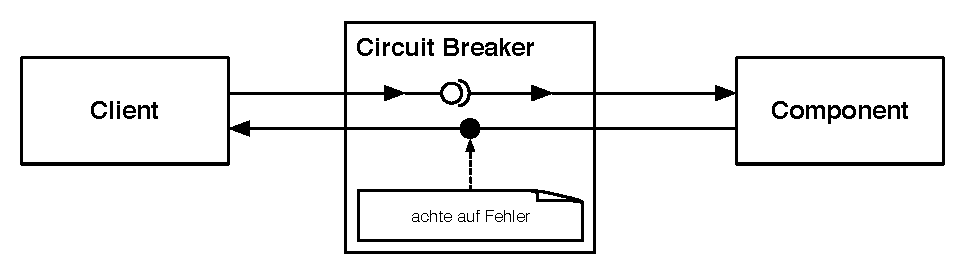
\includegraphics[width=1.0\textwidth]{4-Hauptteil/circuit-breaker/circuit-breaker-closed.eps}
 \caption{Circuit Breaker im geschlossenem Zustand.}
 \label{fig:circuit-breaker-closed}
\end{figure}

Ist die Kommunikation zwischen den Komponenten erfolgreich, bleibt der Circuit Breaker im geschlossenem Zustand. Im Fehlerfall hat der Circuit Breaker die Möglichkeit, den Nachrichtenfluss absichtlich zu unterbrechen. Wird der Nachrichtenfluss unterbrochen, befindet sich der Circuit Breaker im offenem Zustand (siehe Abb. \ref{fig:circuit-breaker-open}). In diesem Zustand wird jede Anfrage sofort mit einer negativen Rückmeldung quitiert --- ohne eine Anfrage verschickt zu haben \cite[S.~94]{nygard_release_2007}.

\begin{figure}[H]
 \centering
 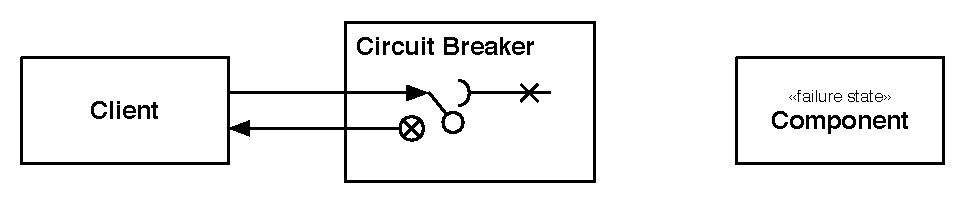
\includegraphics[width=1.0\textwidth]{4-Hauptteil/circuit-breaker/circuit-breaker-open.eps}
 \caption{Circuit Breaker im offenem Zustand.}
 \label{fig:circuit-breaker-open}
\end{figure}

Der Circuit Breaker überwacht Antworten \& Antwortzeiten und protokoliert die Fehler der Kommunikation. Je nach Konfiguration wird die Verbindung, beispielsweise nach 5 fehlerhaften Antworten, absichtlich unterbrochen \cite[S.~94]{nygard_release_2007}.\\
Gründe für den offenen Zustand können beispielsweise Überlastung oder fehlerhaftes Verhalten der angefragten Komponente sein. Überlastung kann dazu führen, dass die Antwortzeiten stetig steigen, bis hin zu Timing oder Omission Failures. Wird die Verbindung unterbrochen, kann sich die überlastete Komponente erholen \cite[S.~203]{kuhn_reactive_2015}. Häufige aufeinanderfolgende Response oder Byzantine Failures können ebenfalls Gründe für den offenen Zustand des Circuit Breaker sein.\\
Nach einer definierten Dauer im geschlossenem Zustand, wird der Circuit Breaker in den halb-offenen Zustand versetzt. In diesem Zustand wird eine Testanfrage zugelassen. Ist diese Anfrage erfolgreich, wird der Circuit Breaker in den offenen Zustand gesetzt. Andernfalls fällt der Circuit Breaker zurück in den geschlossenen Zustand \cite[S.~94]{nygard_release_2007}.\\

Das Pattern eignet sich sehr gut, um die Kommunikation zwischen den Komponenten zu entkoppeln. Somit unterstützt es auch die Isolierung von Komponenten. Kombiniert mit dem Heartbeat Pattern können alle Fehlerkategorien abgedeckt werden. Aus der Sicht des Reactive Manifestos trägt das Circuit Breaker Pattern zur \textit{resilience} bei.

\pagebreak

\pagebreak

\subsection{Fallback Pattern}

\pagebreak

\subsection{Bulkheads Pattern}

\pagebreak

\subsection{Idempotent Receiver}

\pagebreak

\subsection{Saga Pattern}
